\chapter{Requirement Analysis}

We will now investigate some situations where GEX could be used, to establish its requirements and desired features.

\section{Desired Features}

\subsection{Interfacing Intelligent Modules}\label{sec:uses_digital_ifaces}

When adding a new digital sensor or a module to a hardware project, we want to test it first, learn how to properly communicate with it, and confirm its performance. Based on this evaluation we decide whether the module matches our expectations, and learn how to properly connect it. In experimental setups, this connection may be the only thing we need. Sensor data can be collected immediately after gaining access to its communication interface, and the same applies to controlling actuators or other devices.

Several well-known hardware buses have established themselves as the standard ways to interface digital sensors and modules: \gls{SPI}, \gls{I2C} and \gls{USART} (\gls{UART} in asynchronous mode) are some of the most common ones, often accompanied by a few additional \gls{GPIO} lines for features such as Reset, Chip Enable, or Interrupt. There are exceptions where silicon vendors have developed proprietary communication protocols that continue to be used either for historical reasons, or because of their specific advantages. An example is the Dallas Semiconductor 1-Wire bus used in digital thermometers.

Moving to industrial and automotive environments, we encounter various fieldbuses, Ethernet, \gls{CAN}, \gls{HART}, \gls{LIN}, \gls{DALI}, RS-485 (e.g., for Modbus), \gls{mbus}, PLC-BUS, and others. Those typically use transceiver \glspl{IC} and other circuitry, such as \glspl{TVS}, signal filters, or galvanic isolation. 

Since trying to support everything would only distract us from developing a robust core system, we will focus only on the most common interfaces in this work, leaving the more specialized ones to future expansions and add-on boards.

\subsection{Analog Signal Acquisition}

Sometimes, it is necessary to use a traditional analog sensor, to capture a transient waveform, or to just measure voltage. While our main focus lies on digital interfaces, this capability will make the project much more versatile. Nearly all microcontrollers include an \gls{ADC} which we can use to measure input voltages, and, paired with a timer, to records signals varying in time.

Certain tasks, such as capturing transient effects on a thermocouple when inserted into a flame (an example from developing fire-proof materials) demand level triggering, similar to that of oscilloscopes. The converter continuously measures the input voltage and a starts recording the samples only after a set threshold is exceeded. This can be accompanied by a pre-trigger feature where the immediate history is captured when the triggering condition occurs.

\subsection{Analog Signal Output}

An analog signal can not only be measured, but it is often necessary to also generate it. Pairing the analog output and input features, we can perform more complex measurements, such as measuring the frequency response of filters, or the characteristic curves of semiconductor devices.

Generating an analog signal is possible using \gls{PWM} or by a dedicated \gls{DAC} included in many microcontrollers. Higher frequencies or resolution can be achieved with a dedicated external \gls{IC}.

\subsection{Pulse Generation and Measurement}

Some sensors have variable frequency or \gls{PWM} output. To capture those signals and convert them to a more useful digital value, we can utilize the external input functions of a timer/counter peripheral. Those timers have many possible configurations and can also be used for pulse counting or waveform generation.

\subsection{Logic Level Input and Output}

We have covered some more advanced features, but skipped the simplest feature: direct  to \gls{GPIO} pins. Considering the latencies of \gls{USB} and the \gls{PC}'s \gls{OS}, this cannot be used reliably for ``bit banging'' custom protocols, unless they are tolerant to jitter, or very slow; however, we can still accomplish a lot with just changing logic levels---e.g., to control character displays with a parallel interface, or to emulate some interfaces that include a clock line. As mentioned in \cref{sec:uses_digital_ifaces}, many digital sensors and modules use plain \glspl{GPIO}, in addition to the communication bus, for out-of-band signaling or features like chip select or reset.

\section{Connection to the Host Computer}

\subsection{Communication Interface}

\gls{USB} shall be the primary way of connecting the module to a host \gls{PC}. Thanks to \gls{USB}'s flexibility, the \gls{MCU} can present itself as any kind of device, or even multiple devices at once.

The most straightforward method of interfacing the board is by passing binary messages in a fashion similar to \gls{UART}. This is possible either using a ``Virtual COM port'' driver, or through raw access to the corresponding \gls{USB} endpoints. Using raw access avoids potential problems with the \gls{OS}'s driver interfering or not recognizing the device correctly; on the other hand, having GEX appear as a serial port makes it easier to integrate into existing platforms that have good serial port support (such as National Instruments LabWindows~CVI, Visual C++ applications, or VBA macros).

GEX may be used with development boards lacking a ``User'' \gls{USB} connector, such as STM32 Nucleo. In this case, either the board can be customized, or we use the built-in \gls{USB}/\gls{UART} converter; that requires the communication interface to be available also through hardware \gls{UART}. Another use-case is in battery-powered setups where wired access is not possible or practical. For those cases the ideal solution is a wireless connection.

\subsection{Configuration Files}

The module must be easily reconfigurable. Given the settings are almost always going to be tied to the connected external hardware, it would be practical to have an option to store them permanently in the microcontroller's non-volatile (flash) memory.

We can load those settings into GEX using the serial interface, which also makes it possible to reconfigure it remotely through the wireless connection. With USB, the board may additionally appear as a mass storage device and expose the configuration as text files. This approach, inspired by \mbed's mechanism for flashing firmware images to development kits, avoids the need to create a configuration \gls{GUI}, instead using the built-in applications of the \gls{PC} \gls{OS} to view and edit files.

\section{An Overview of Planned Features}

Summarizing the preceding discussion, we obtain the following list of features to implement in the GEX firmware:

\begin{itemize}
	\item \textbf{Hardware interfacing functions}
		\begin{itemize}
			\item I/O pin direct access (read, write), pin change interrupt
			\item Analog input: voltage measurement, isochronous sampling
			\item Analog output: DC level, waveform generation
			\item Frequency, duty cycle, and pulse length measurement
			\item Pulse and \gls{PWM} generation
			\item Digital interfaces: \gls{SPI}, \gls{I2C}, \gls{UART}/\gls{USART}, and 1-Wire
		\end{itemize}
	\pagebreak[0]
	\item \textbf{Communication with the host computer}
		\begin{itemize}
			\item \gls{USB} connection as virtual COM port, or with direct endpoint access
			\item Connection using plain \gls{UART}
			\item Wireless link
		\end{itemize}
	\item \textbf{Configuration}
		\begin{itemize}
			\item Fully reconfigurable, temporarily or permanently
			\item Settings stored in INI files
			\item File access through the communication interface or a virtual mass storage device
		\end{itemize}
\end{itemize}

\section{Microcontroller Selection}

As discussed in \cref{sec:expected_outcome}, the project should be based on microcontrollers from the STM32 family. We chose the STM32F072 for the initial hardware and firmware design due to its low cost, advanced peripherals, and the availability of development boards. The firmware can be ported to other \glspl{MCU} later (e.g., to STM32L072, STM32F103 or STM32F303).

The STM32F072 is an \armcm device with 128\,KiB of flash memory, 16\,KiB of \gls{RAM}, and running at 48\,MHz. It is equipped with a \gls{USB} Full Speed peripheral block, 12-bit \gls{ADC} and \gls{DAC}, a number of general-purpose timers/counters, and peripheral blocks like SPI, I$^2$C, or USART. It supports a crystal-less \gls{USB} mode, using the \gls{USB} SOF packet to synchronize an internal 48\,MHz RC oscillator; naturally, a real crystal resonator will provide better timing accuracy.

To effectively utilize the time available for this work, only the STM32F072 firmware will be developed, while making sure the planned expansion to other modules and by adding additional features is as straightforward as possible.

\section{Form Factor Considerations} \label{sec:formfactors}

While the GEX firmware can be used with existing evaluation boards from ST Microelectronics (\cref{fig:discovery}), we wish to design and realize a few custom hardware prototypes that will be smaller and more convenient to use.

Three possible form factors are drawn in \cref{fig:ff_sketches}. The use of a common connector layout and pin assignments, here Arduino and Raspberry Pi, makes it possible to reuse add-on boards from these platforms. Copying the physical shape and connector layout of another device further allows us to reuse existing enclosures designed for it.

\begin{figure}[h]
	\centering
	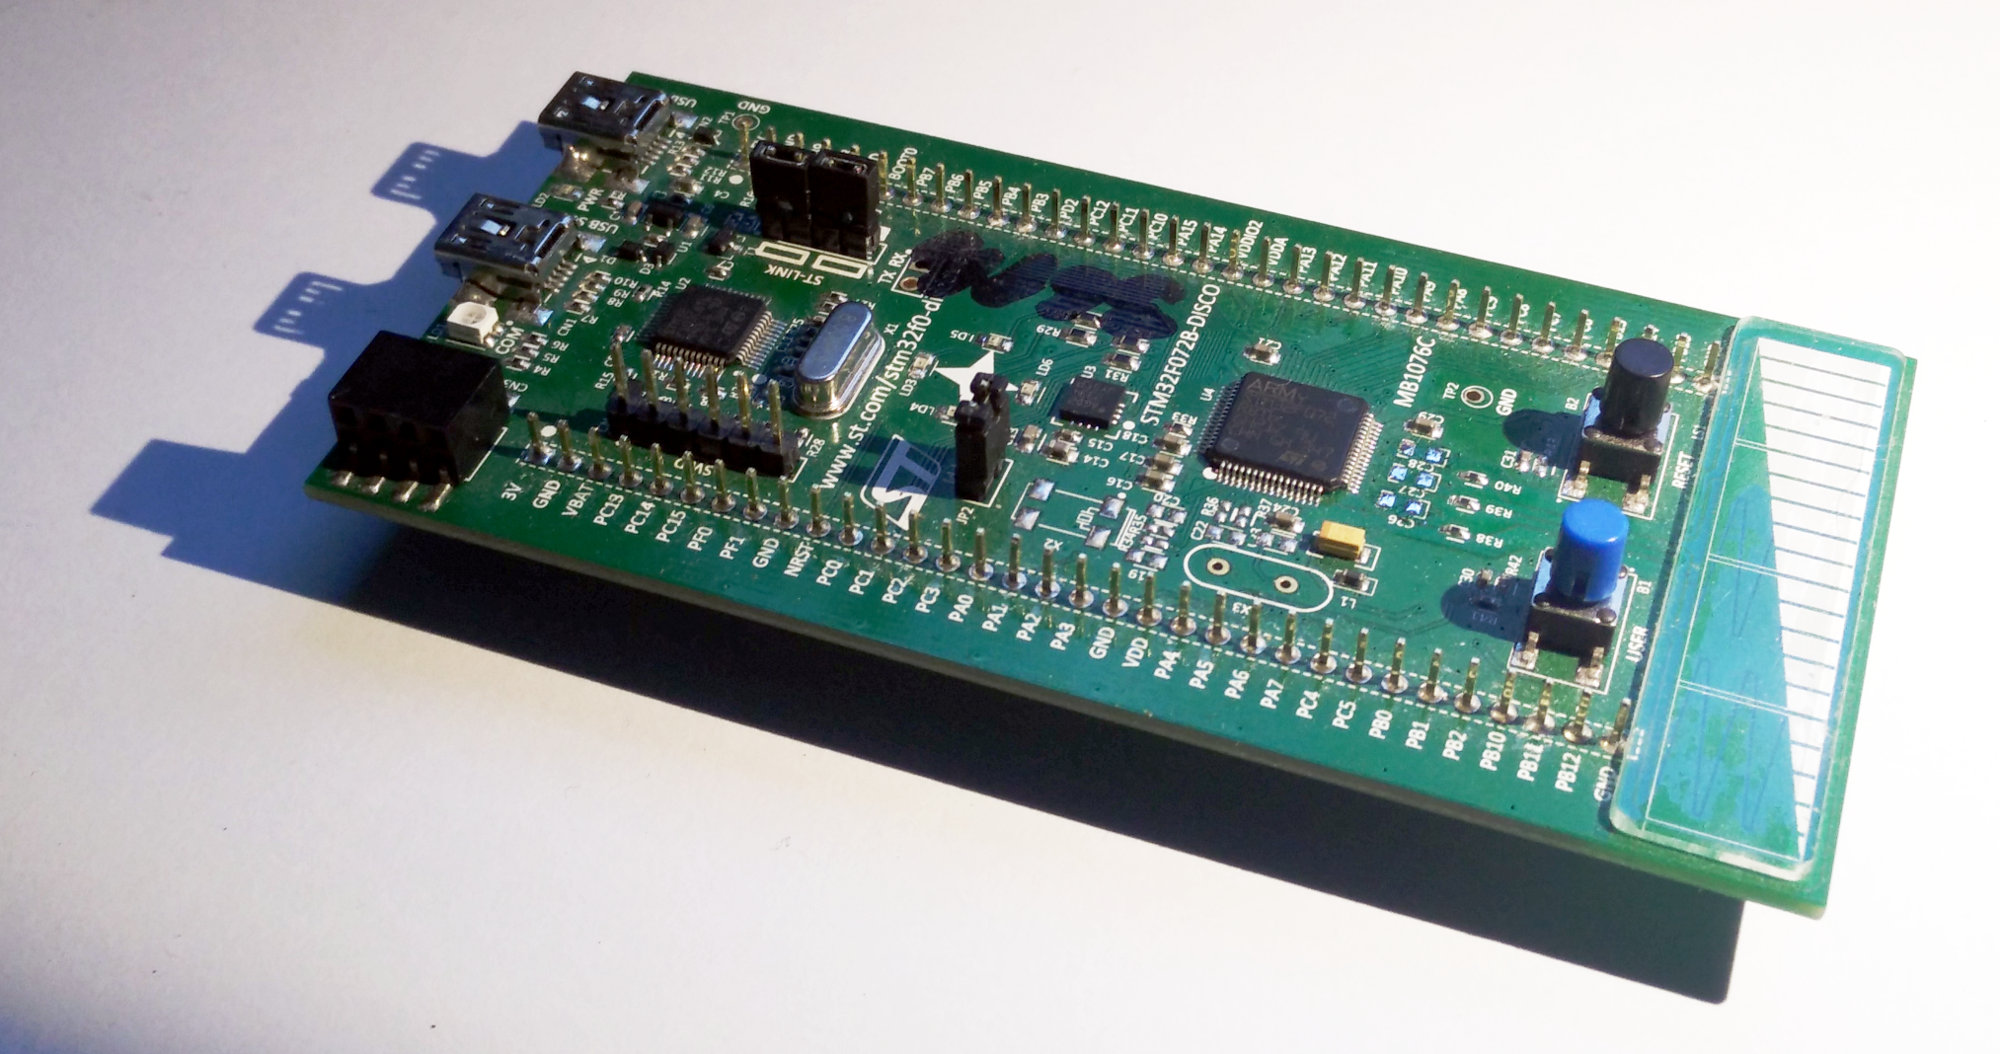
\includegraphics[width=0.7\textwidth] {img/disco072.jpg}
	\caption[Discovery board with STM32F072]{\label{fig:discovery}STM32 Discovery development board with the STM32F072 microcontroller}
\end{figure}

\begin{figure}[h]
	\centering
	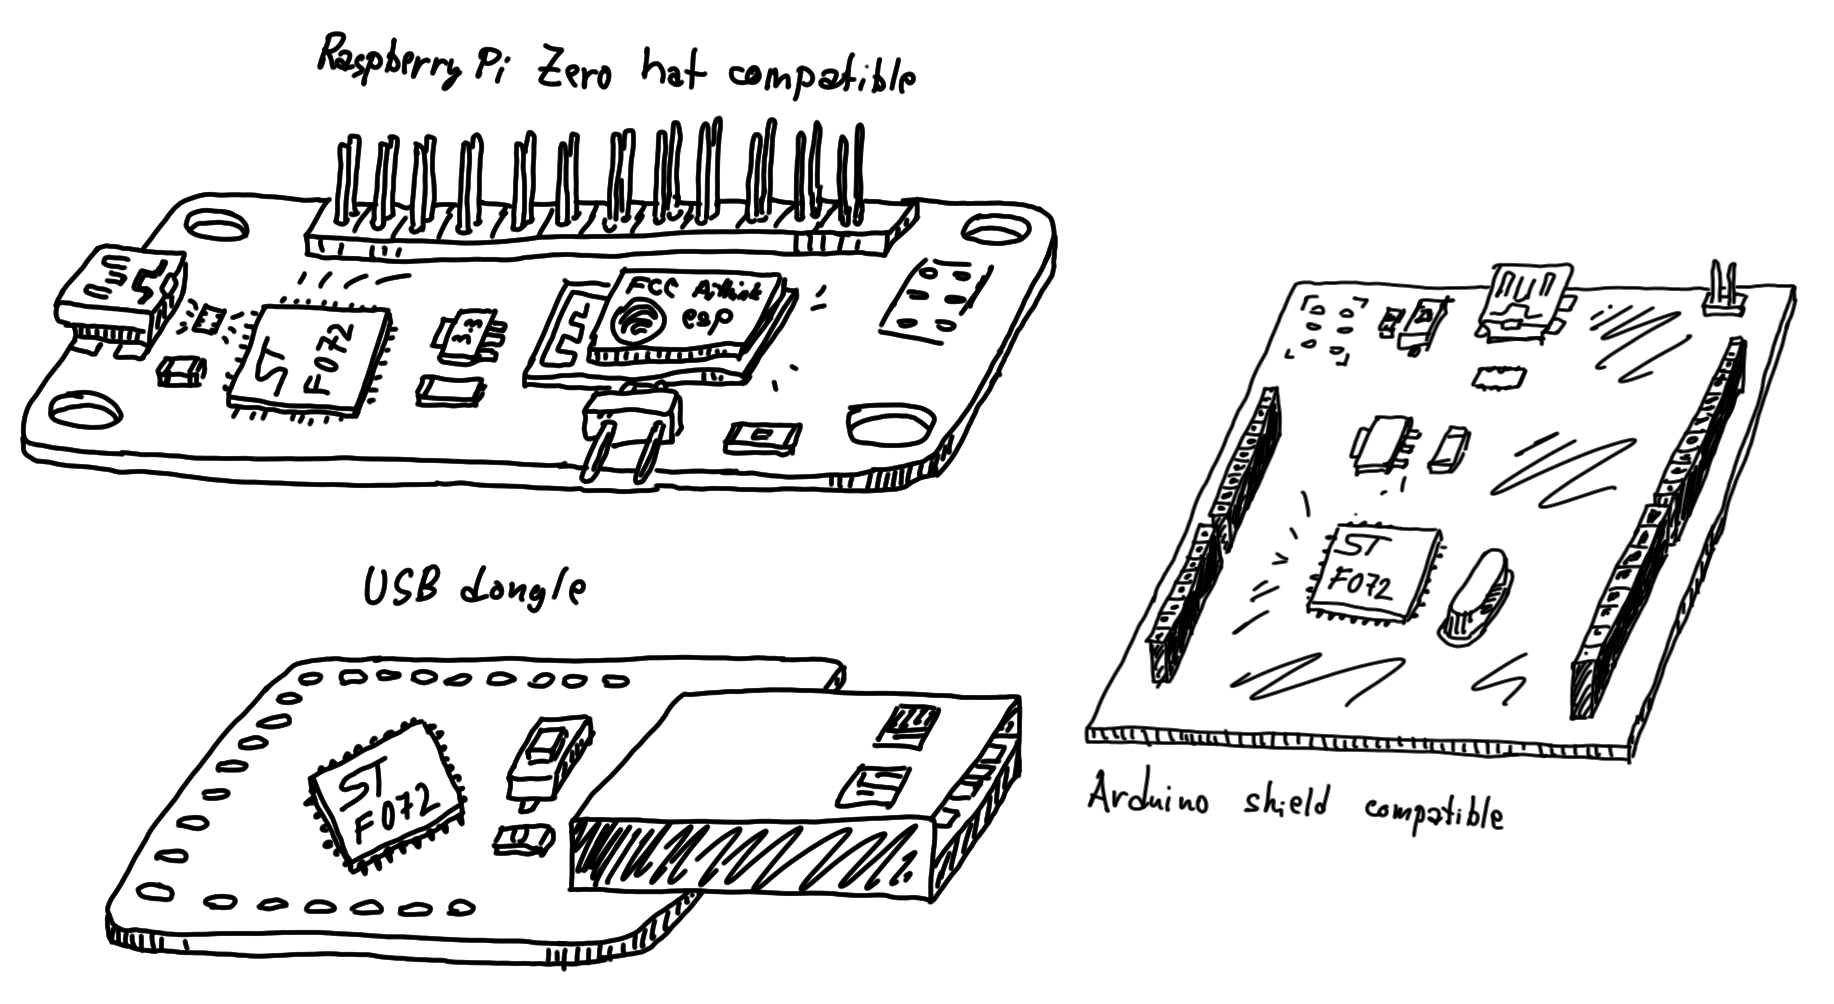
\includegraphics[width=\textwidth] {img/gex-ff-sketches.png}
	\caption[Form factor sketches]{\label{fig:ff_sketches}A sketch of three possible form factors for the GEX hardware realization}
\end{figure}









